\chapter{The Quantum Dot} \label{sec:QuantumDot} \index{Quantum Dot}

	Quantum dots are atomic structures (usually spherical) that have a size of about 1-10nm in diameter. They are often referred to as \glspl{NC}, though this
	term is more general and includes also other shapes and morphologies, which might extend to several $\mu$m, such as rods, wires etc.
	Figure \ref{fig:QDshapes} gives some examples of possible shapes and morphologies, that are possible with nowadays technologies.
	
	\glspl{QD} are possible with various materials such as metals, semiconductors and compounds. According to their size and material,
	a \glpl{QD} can contain just a few or millions of atoms. A 10nm cube of GaAs contains for example 40,000 atoms \cite{SalehTeich}.
	
	The properties of \glspl{QD} are strongly dependent on their size. Figure \ref{fig:QDTheory} illustrates this effect for a semiconductor \gls{QD}.
	Under ultraviolet excitation, the \glspl{QD} emit light according to their size and therefore band gap.
	
	\begin{figure}[htbp]
		\begin{minipage}[t]{0.49\textwidth}
			\centering
			\includegraphics[width=\textwidth]{Fig/QDshapes.jpg}
			\caption{Examples of inorganic nanomaterials with different
							 shapes and morphologies synthesized by colloidal chemistry:
							 (a) PbSe cubes; (b) CdTe tetrapods; (c) PbSe nanowires and
							 (d) hollow iron oxide nanoparticles.
							 {\scshape Source:} \cite[p.394]{Talapin}}
			\label{fig:QDshapes}
		\end{minipage}
		\hfill
		\begin{minipage}[t]{0.49\textwidth}
			\centering
			\includegraphics[width=\textwidth]{Fig/QDcolor.jpg}
			\caption{This photograph shows the size-dependent \gls{PL} of the quantum dots. The particles with the smallest ($\sim$1.7nm)
							 CdSe cores emit blue and those with the largest cores ($\sim$5nm) emit red.
							 {\scshape Source:} \cite[p.393]{Talapin}}
			\label{fig:QDTheory}
		\end{minipage}
	\end{figure}			

	\paragraph{Basic physics of the Quantum Dot}
		For bulk materials the band gap \index{Band gap} is a fixed parameter, that specifies the type of material. But when a particle gets smaller and reaches
		a size of about 10nm this will not be the case anymore. The band gap is than depending on the size of this particle (\glspl{NC}). As
		the mobility of the charge carriers (electrons, holes) is very limited in all three dimensions in the quantum dot, the energy levels
		are not continuous, but instead discrete.
		This phenomenon is called the {\it quantum size effect}.
		
		The band gap \index{Band gap} of a spherical \gls{QD} of radius $R$ is then approximately:
		\begin{equation}
			E_{g} \approx E_{g,0} + \frac{\hbar^2 \pi^2}{2 m_{eh} R^2}
			\label{eq:Bandgap}
		\end{equation}
		where $E_{g,0}$ denotes the band gap of the bulk material and $m_{eh}$ is obtained through the effective masses of electrons and holes $m_{e,p}$:
		\begin{equation}
			m_{eh} = \frac{m_e m_h}{m_e + m_h}
			\label{eq:QuantumBox}
		\end{equation}
		
		\begin{figure}[htbp]
			\centering
			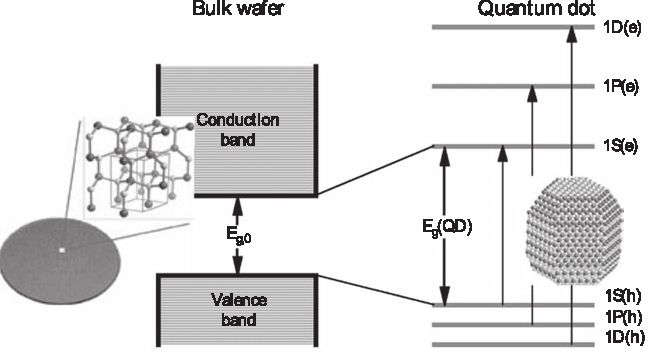
\includegraphics[width=0.4\textwidth]{Fig/QDTheory.pdf}
			\caption{The left illustration shows the band structure of a bulk semiconductor with energy band gap $E_{g,0}$,
							 whereas the the right one illustrates the discrete energy levels of a \gls{QD} and its energy gap $E_{g}(QD)$.
							 {\scshape Source:} \cite[p.3]{Klimov}}
			\label{fig:QDTheory}
		\end{figure}
		
		
		We will see later in chapter \ref{sec:BandGapAnalysis} that the \gls{QD} absorption spectrum \index{Absorption spectrum} as shown in figure \ref{fig:QDTheory}(c) is not really discrete; as it is
		not possible to fabricate \glspl{QD} that are perfectly equal in size, this results in a broadening of the spectrum.
		The energy gap increases for decreasing \gls{QD} sizes, because more energy is required to confine the electron to a smaller volume.
		This is caused by Heisenberg's uncertainty principle \index{Heisenberg uncertainty principle}, which says, that if we want to locate a particle of effective mass $m$ (for example an electron),
		on an x-axis within an interval	$\Delta x$, we can only make an uncertain prediction of its impulse. If the spatial region gets smaller, the uncertainty
		of the impulse will	increase.
		\begin{equation}
			\Delta p_{x} \sim \frac{\hbar}{\Delta x}
		\end{equation}
		This adds to the kinetic energy of the free particle, which is called the confinement \index{Confinement} energy \index{Confinement!Energy}, that has an significant impact, if it gets bigger
		than the thermal energy of the particle.
		\begin{equation}
			E_{confinement} = \frac{(\Delta p_{x})^2}{2 m} \sim \frac{\hbar^2}{2 m (\Delta x)^2} > \frac{1}{2} k_{B} T
		\end{equation}
		From this we can conclude, that the quantum size effect is relevant if
		\begin{equation}
			\Delta x < \sqrt{\frac{\hbar^2}{m k_{B} T}}
		\end{equation}
		Table \ref{tbl:ConfinedStr} shows 4 possible confinement structures\index{Confinement!Structure}, which are illustrated in Figure \ref{fig:ConfinedStr} with their
		characteristic energy levels \index{Energy level} in	the conduction band.

		\begin{figure}[htbp]		
		\centering
		\includegraphics[width=0.5\textwidth]{Fig/ConfinedStructures.pdf}
		\caption{Schematic representation of quantum wells, wires and dots (left).
						 The generic shape of the density of states function for electrons in the
						 conduction band of a semiconductor with band gap $E_{g}$ is shown for each
						 type of the structure (right).
						 {\scshape Source:} \cite[p.143]{Fox}}
		\label{fig:ConfinedStr}
	\end{figure}
		
		\begin{table}[htbp]
		\centering
			\begin{tabular}{lccc}
				Structure											&	Quantum				&	\# of free		&	Electron						\\
																			&	confinement		&	dimensions		&	density of states		\\
				\hline
				Bulk													&	none					&	3							&	$\propto E^{1/2}$		\\
				Quantum well/superlattice			&	1-D						&	2							&	$\propto E^{0}$			\\
				Quantum wire									&	2-D						&	1							&	$\propto E^{-1/2}$	\\
				Quantum dot/box								&	3-D						&	0							&	discrete						\\
			\end{tabular}
			\caption{Number of degrees of freedom tabulated against the dimensionality of the quantum confinement.
							 The final column shows the functional form of the density of states for free electrons.
							 {\scshape Source:} \cite[p.142]{Fox}}
			\label{tbl:ConfinedStr}
		\end{table}
	
	\paragraph{Fabrication techniques of \gls{QD}}
	
		A lot of different ways to make \glspl{QD} have been developed. Research efforts are made to create
		more efficient \glspl{QD} and new shapes and morphologies. As \glspl{QD} are more and more interesting for various commercial applications,
		low costs play an important factor. The colloidal chemistry has made a major contribution, as it offers low energy
		synthesis of \glspl{NC}/\glspl{QD} using very simple and affordable laboratory equipment.		
		In the next chapter we will briefly discuss the mentioned technique, by giving a short overview
		that avoids the use of chemical terms as much as possible, rather than a detailed disquisition, as this is a research field on its own.
		
		Some other methods are listed below.
	
		\begin{tabularx}{\textwidth}{Xl}
			{\bf Physical methods}														&	{\bf Characterization}										\\
			Molecular-beam-epitaxy (MBE)											& High-energy-input, expensive apparatus,
																													used	for \glspl{QD}											\\
			Metalorganic-chemical-vapor-decomposition (MOCVD)	&	High-energy-input, used for \glspl{QD}		\\
			Vapor-liquid-solid (VLS)													&	High-energy-input, used for quantum wires	\\
			Electron-beam lithography													&			\\
																												&			\\
			{\bf Chemical methods}														&	{\bf Characterization}										\\
			Colloidal chemical synthesis of crystalline
			semiconductor nanoparticles												& Low-energy-input, wet chemistry,
																													used for various structures								\\
		\end{tabularx}
	
		
		
	\paragraph{Applications}
		
		In biology and chemistry \glspl{QD} are used as spectral tags that are attached to molecules, making their position visible for identification
		under optical illumination. In the past, one used organic dyes, but compared to \glspl{QD} the sharpness of emission lines is not as good.
		
		In electronics, \glspl{QD} are used to increase the efficiency of lasers \cite{SemiconductorCD}, everyday light sources and solar cells.
		Furthermore they are used	in broadband \gls{LED}, memory elements, flexible displays, photodetectors.
		
		We have to add that a lot of these applications are still developed in research institutions and are not yet available for commercial use.
		
		Although the applications seem impressive and will probably motivate new technologies, there are reasonable concerns about these nanoscale
		particles. Some of the materials are toxic and through the small sizes it is unclear what might happen if the particles end up in living
		organisms or generally speaking, into the the environment.
		For more interested readers, we recommend the following paper for further reading: \citeauthor{Hardman} \citetitle{Hardman} \cite{Hardman}.